\chapter{The PyBayes Library}

In this chapter the PyBayes library that is being developed with the aim to fulfil the requirements
posed in the previous chapter (p. \pageref{sec:Requirements}) is presented. After a brief introduction
the library design, which builds on the performed software analysis, is shown and discussed.
Various development practices used are later examined and the chapter is concluded by a performance
comparison of various implementations of the Kalman filter (from PyBayes and BDM) benchmarked under
4 different implementation environments.

\section{Introduction to PyBayes}

PyBayes\footnote{the name PyBayes had been previously used for an unrelated project dealing with
Bayesian networks by Denis Deratani Maua, who later proclaimed the project dead and allowed us
to use the name.}
is a Python/Cython library for recursive Bayesian estimation actively developed by the
author of this text, a result of the software analysis carried-out. The development happens publicly
and openly using the git\footnote{\url{http://git-scm.com/}} version control system on the
GitHub\footnote{\url{http://github.com}} source-code hosting service at the address
\url{http://github.com/strohel/PyBayes} that also serves as the home page of the project; PyBayes is
also accessible from the Python Package Index (PyPI).\footnote{\url{http://pypi.python.org/pypi/PyBayes}}
\ifattachements
	Additionally, the snapshot of version 0.3 is available on the enclosed CD-ROM.
\fi
PyBayes is a free/open-source software licensed under the GNU GPL\footnote{GNU General Public
License: \url{http://www.gnu.org/licenses/gpl.html}}, version 2 or later. Version 0.3 of PyBayes is
described in this text; we expect PyBayes to evolve in future and thus some claims present this
chapter may become outdated. All currently planned future changes are however mentioned at
appropriate places.

The goal of PyBayes is to provide a Python library that satisfies the posed requirements, is very
convenient to develop with even when prototyping novel algorithms, but fast enough to be deployed in
production. Library design should be object-oriented and very clean to be well comprehensible.
In order to achieve both of these usually contradicting demands, PyBayes uses a special
technique where the same source code can be interpreted by Python as usual (giving all advantages
of Python) or compiled using Cython which makes use of additional \emph{augmenting files} that are present
in sources to provide static
type declarations to performance-critical code-paths; PyBayes thus employs Cython's \emph{pure Python
mode}. The Cython build is currently 50\% to 200\% faster than Python depending on the algorithm and
level of optimisation applied to it, see \autoref{sec:PyBayesPerformance} (p.~\pageref{sec:PyBayesPerformance})
for example measurements. PyBayes' \verb|setup.py|, the use of which is the standard way to install
Python packages, automatically detects whether Cython is installed on the system and uses it when
possible. NumPy's \verb|ndarray| (N-dimensional array) of Python \verb|floats|\footnote{Python
\verb|float| (\verb|numbers.Real|) corresponds to C \verb|double|} is used as principal
numeric type for vectors and matrices for its low overhead, convenience and interoperability.

PyBayes sources are maintained to be compatible with Python versions 2.5, 2.5 and 2.7; Python 3
compatibility can achieved using the 2to3\footnote{\url{http://docs.python.org/library/2to3.html}}
automatic code conversion tool, the sources are kept to be convertible without interaction
(CPython's \verb|-3| command-line can be used for this task). To promote code readability, coding
style prescribed by the PEP 8\footnote{Python Enhancement Proposal 8:
\url{http://www.python.org/dev/peps/pep-0008/}} is followed when feasible.

The sections below present the library design and explain some decisions taken during development;
they complement the PyBayes API Documentation available on-line at \url{http://strohel.github.com/PyBayes-doc/}%
\ifattachements%
, in the appendix (p. \pageref{chap:APIDocs}) and on the enclosed CD-ROM
\fi
which is a reference guide intended for PyBayes users.

All class diagrams in this text utilise standard UML\footnote{Unified Modelling Language:
\url{http://www.uml.org/}} notation and are not an exhaustive reference of all classes, members and
methods --- they rather illustrate the API Documentation; inherited attributes and methods are not
shown in diagrams. Unless noted otherwise, all references to
files and folders in this chapter refer to the respective files/folders in the PyBayes source code
repository.\footnote{\url{http://github.com/strohel/PyBayes}} Python software nomenclature is used,
most notably the following terms:
\begin{description}
	\item[module] a file with .py extension (but denoted without it) that contains Python code and
		has its own namespace.
	\item[package] a folder that contains above modules and possibly other packages; package
		namespace is identical with its \verb|__init__| module that has to be present.
\end{description}

\section{Library Layout}

The source code of PyBayes is arranged as follows:

\noindent\begin{tabular}{rp{\textwidth-92pt}}
\verb|doc/|      & control files for generating documentation (see also \autoref{sec:PyBayesDocsTests}). \\
\verb|examples/| & auxiliary scripts and benchmark sources. \\
\verb|pybayes/|  & PyBayes Python package; the actual implementation is located in this package. \\
\verb|scratch/|  & miscellaneous and temporary files. \\
\verb|thesis/|   & source code of this text. \\
\verb|tokyo/|    & source code of the Tokyo project, bundled with PyBayes (see \autoref{sec:PyBayesWrappers}). \\
\verb|COPYING|   & the text of GNU GPL v2, the PyBayes license. \\
\verb|HACKING.rst| & a guide for PyBayes developers; can be viewed as plain-text. \\
\verb|README.rst|  & general information and installation instructions. \\
\verb|setup.py|    & setup script, a tool to build and install PyBayes. \\
\end{tabular}

The \verb|pybayes| package, the most important part that forms the actual PyBayes library, contains
3 supportive packages that are considered private to PyBayes (that may change without notice), and
2 following modules that form the public API of the library (overview shown in \autoref{fig:DiaPyBayes}):
\begin{description}
	\item[pdfs] module contains a framework of {\pdfs} and related classes.
	\item[filters] module contains Bayesian filters.
\end{description}

\begin{figure}[h]
	\centering
	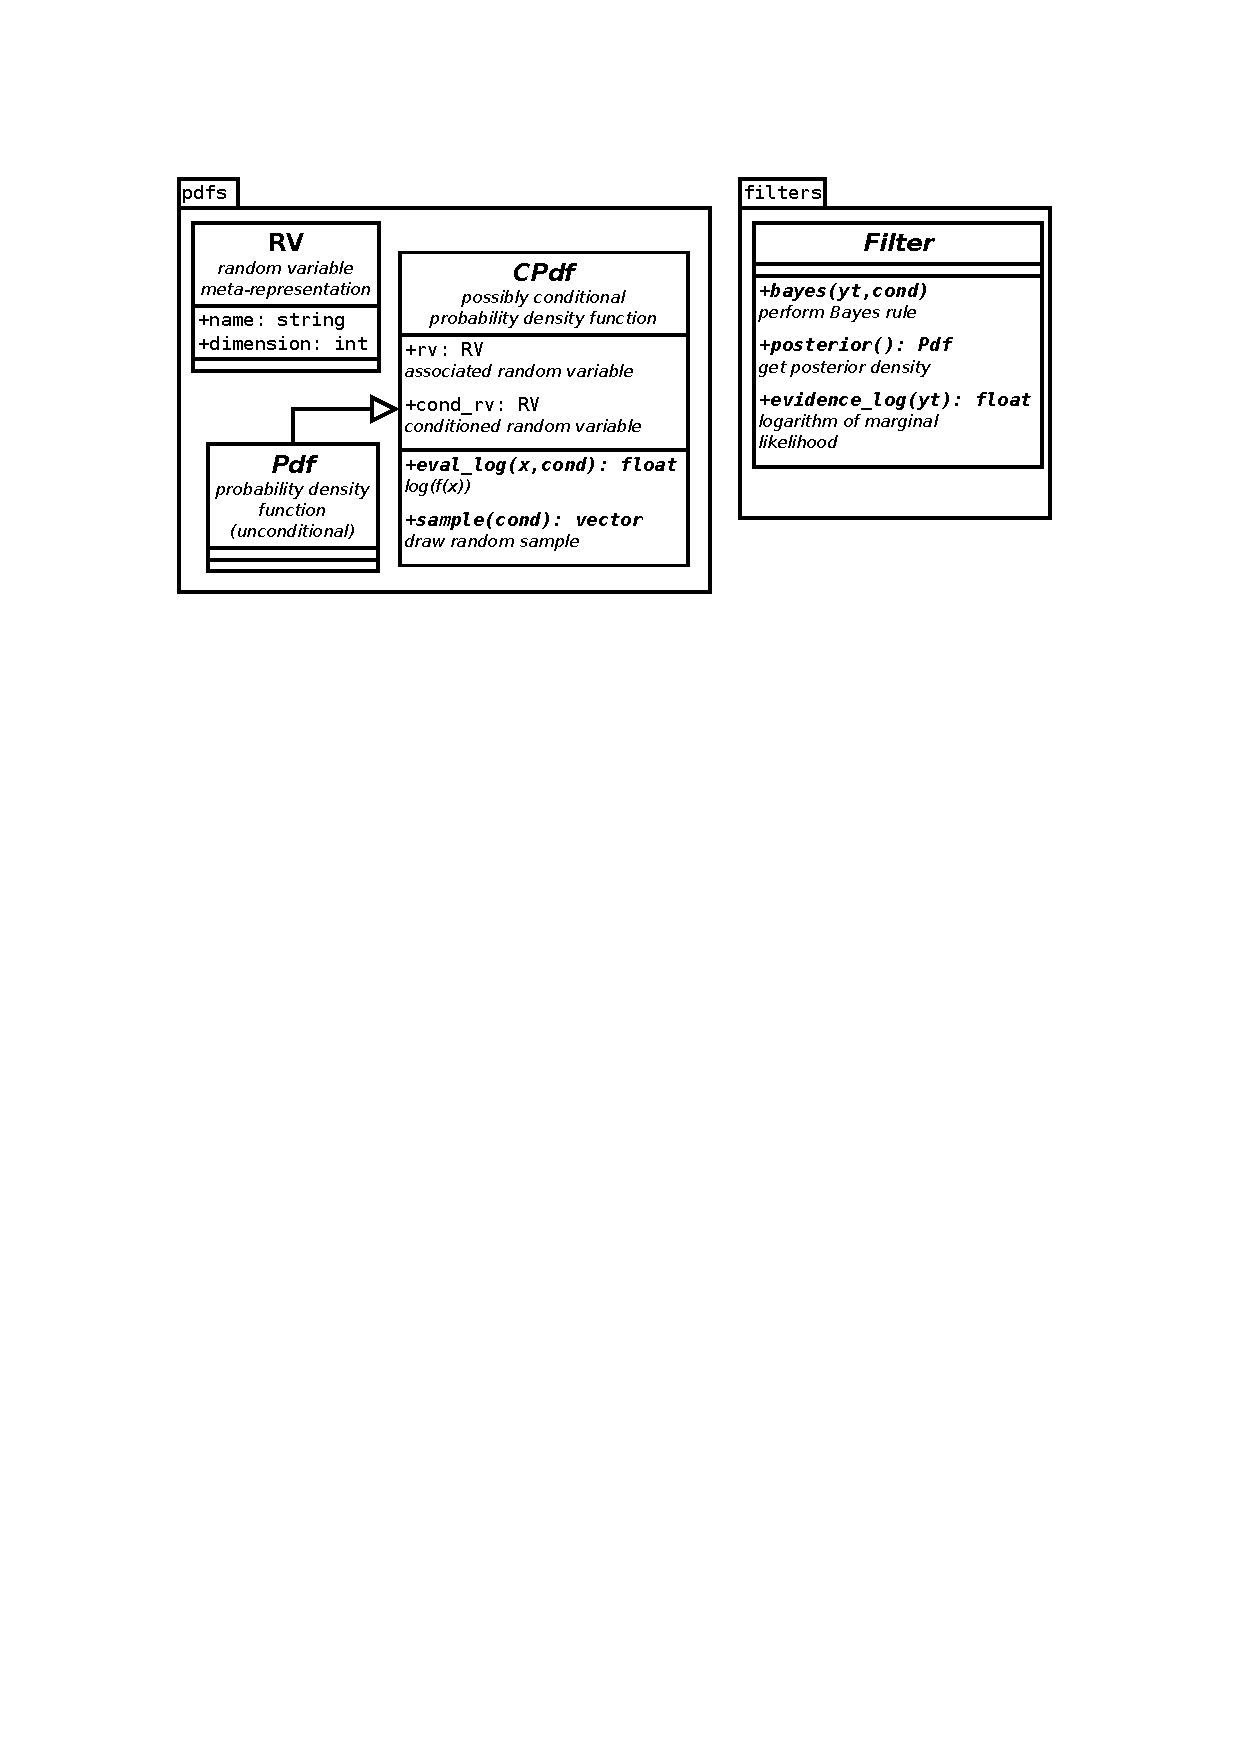
\includegraphics[width=\textwidth,keepaspectratio=true,clip=true,trim=3cm 196mm 3cm 3cm]{./diagrams/PyBayes.pdf}
	\vspace{-8mm}
	\caption{High-level overview of the PyBayes library; simplified}
	\label{fig:DiaPyBayes}
\end{figure}

\subsection{Probability Density Functions}

Probability density functions have central role in the theory of Bayesian filtering and thus should
receive great attention during library design. Probability density functions should be both flexible
and lightweight as copying them is needed for example in the marginalized particle filter. In PyBayes
{\pdfs} are multivariate (even distributions that cannot be generalised to multiple dimensions take
singe-valued vectors as parameters for consistency and easier static typing).

2 basic categories of {\pdfs} can be distinguished from the implementation point of view:
unconditional ones whose statistics are fixed once the distribution is constructed and conditional
{\pdfs} whose statistics depend on a free parameter; depending on one's standpoint, unconditional
{\pdfs} may be viewed as a subclass of unconditional ones (that would have additional method
\verb|set_condition(cond)| or similar) or the other way around where unconditional {\pdf} is viewed
as a specialisation of the conditional ones with a restriction that condition is empty.
The latter approach is used by PyBayes for being less error-prone in our belief.
Alternatively, conditional and unconditional densities could be unrelated (impractical in our case)
or unified in one class without specifying conditionality (in fact, PyBayes is not far from this).

All {\pdfs} are represented using an abstract class \emph{CPdf} that provides interface for querying
random variable and conditioning variable dimensions (methods \verb|shape()| and \verb|cond_shape()|),
for computing expected value and variance (methods \verb|mean()| and \verb|varience()|) that take
condition as a parameter, for computing natural logarithm of the {\pdf} value in a given point
(\verb|eval_log()|) and for drawing random samples (\verb|sample()|), both also accepting condition
in parameters. A few support methods for use by subclasses not are provided to reduce code
duplication, these aren't discussed here. The CPdf class also holds references to random variable
and conditioning variable descriptions (attributes \verb|rv| and \verb|cond_rv|) which are talked 
bout in the next chapter. By convention \verb|rv| and \verb|cond_rv| to a valid \emph{RV} object
that can, however, signify ``empty random variable''.

The \emph{Pdf} is a very thin subclass of CPdf providing an implementation of the \verb|cond_shape()|
that returns zero to signify empty condition; by convention, Pdf subclasses also should set
\verb|cond_rv| to ``empty random variable''. The function of the Pdf class is therefore rather
semantic than technical distinction between conditional and unconditional {\pdfs}.

Outline of {\pdf} prototypes is shown in the \autoref{fig:DiaPdfs}.

\begin{figure}[h!]
	\centering
	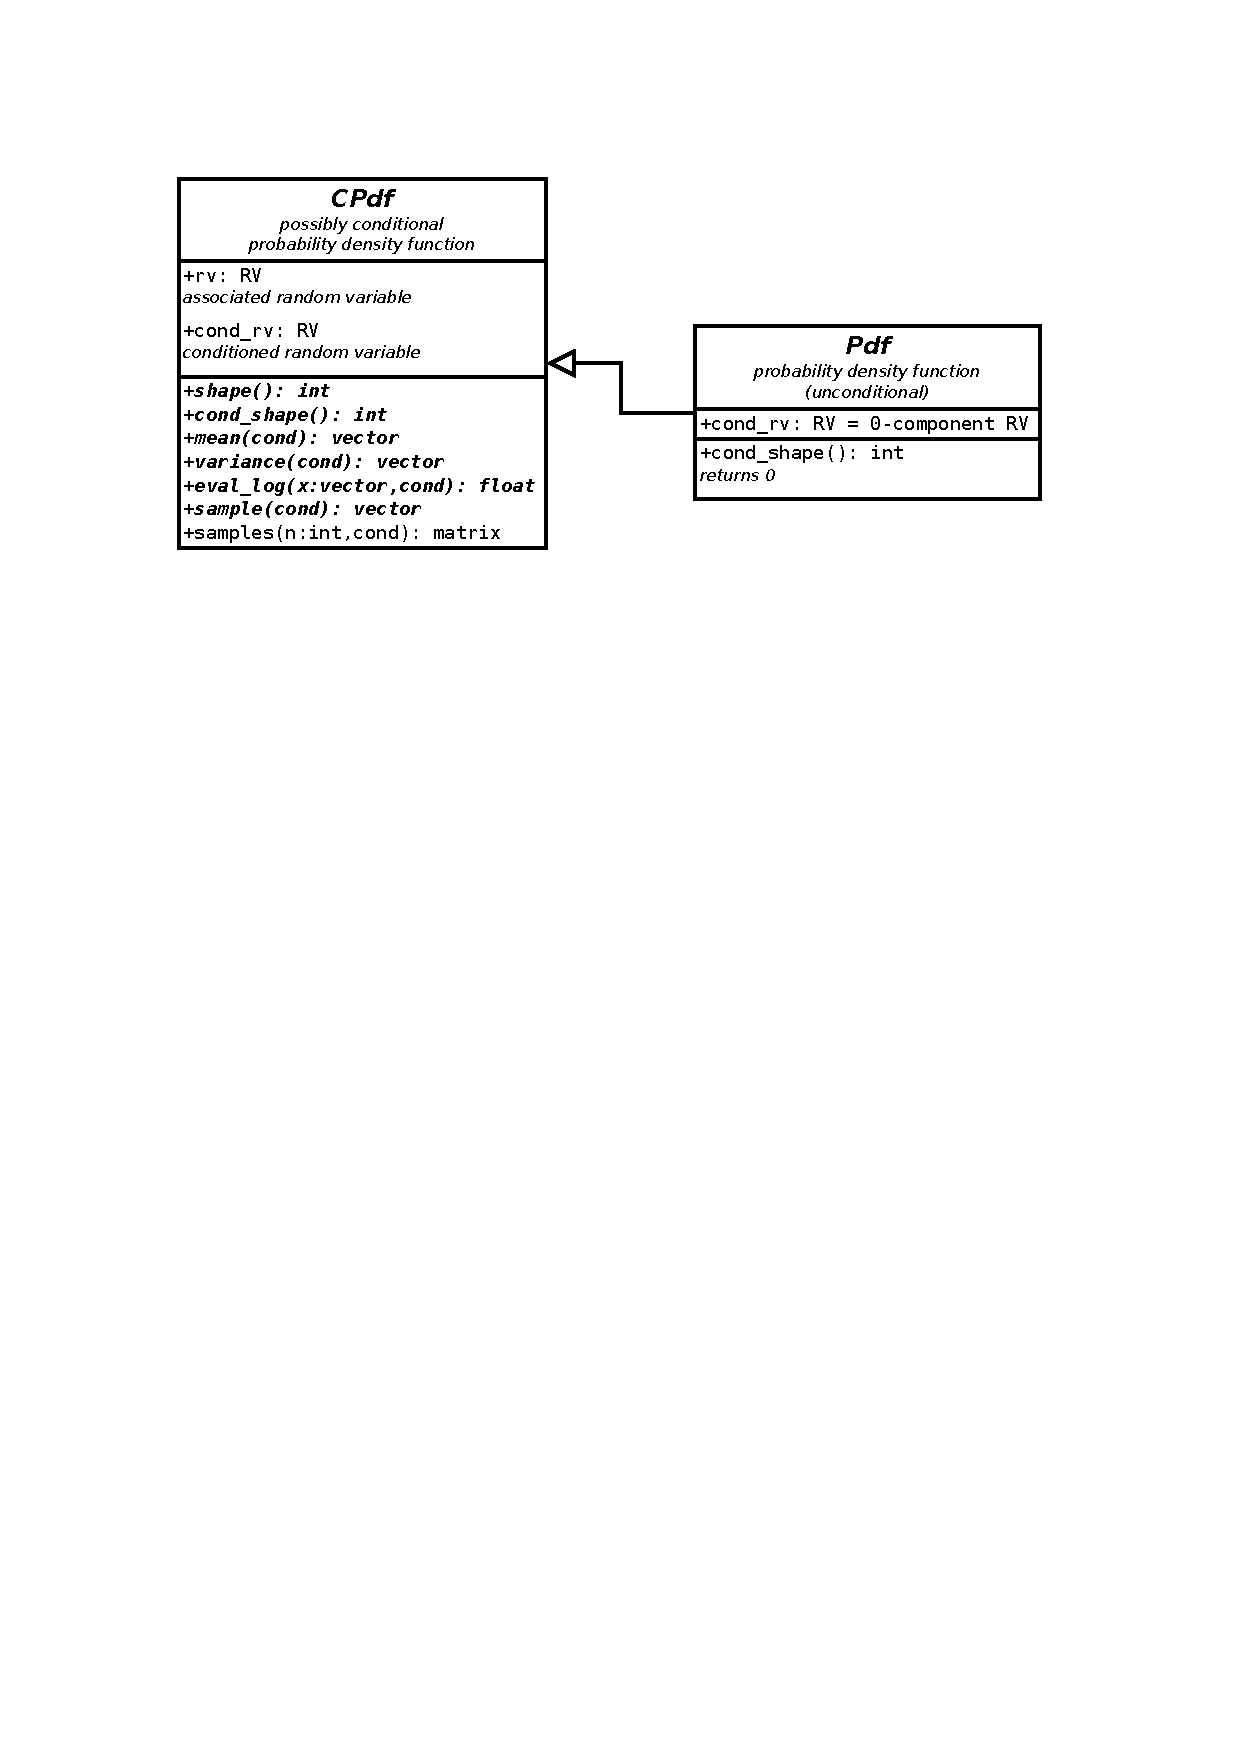
\includegraphics[width=\textwidth,keepaspectratio=true,clip=true,trim=3cm 204mm 3cm 3cm]{./diagrams/pdfs.pdf}
	\vspace{-8mm}
	\caption{Class diagram of the {\pdf} prototypes}
	\label{fig:DiaPdfs}
\end{figure}

\subsection{Random Variable Meta-representation}

In mathematics, the relation between random variables and {\pdfs} is follows: a {\pdf} is associated
to a random variable, e.g. ``random variable \(X\) is normally distributed''. This is impractical in
software (should drawing a million bare samples produce a million copies of a random variable?) but
the relation between random variables and {\pdfs} couldn't be entirely dropped without a substitution,
as illustrated in the following example.

The chain rule for {\pdfs} is heavily used in Bayesian filtering and should be adequately supported
by software. While simple cases can be represented without problems, when for example \(p(a,b|c,d)\)
from \eqref{eq:ProdCPdf} is desired to be represented, additional information have to be supplied by
the user (programmer) so that correct data-flow can be established (e.g. the order of conditioning
variables of \(p_1\) cannot be determined automatically).
\begin{equation} \label{eq:ProdCPdf}
	p(a,b|c,d) = p_1(a|c,b) p_2(b|d)
\end{equation}

The first option would be to force the user to specify the relations between distributions manually
(for example using a form of directed acyclic graph); we believe that it is however error-prone
and inconvenient. The other method is to make the association the other way around --- random
variables would be associated to {\pdfs}, in our example above \(p_1\) would contain an information
that it has random variable \(a\) and conditioning variables \(c,b\).

The second approach is used in PyBayes even though it brings some computational overhead (that we
think is worth the simplicity it brings). As mentioned in the previous section, the CPdf class has
\verb|rv| and \verb|cond_rv| attributes that hold instances of the \emph{RV} class.

The RV class is essentially a list of ``random vector components'' represented using the
\emph{RVComp} class. RV provides a few methods to test relationships between 2 random vectors
(whether a RV is subset of another RV etc.) and one notable method, \verb|indexed_in()|. Suppose
that RV \(x\) has components \((x_1, x_2 \dots x_n)\) and RV \(y\) is a subset of \(x\) and contains
components \((x_{i_1}, x_{i_2} \dots x_{i_m})\); \verb|y.indexed_in(x)| then returns an index array
\((i_1, i_2 \dots i_m)\) which is suitable for NumPy array indexing methods.

The RVComp class is a simple container for the optional \verb|name| and \verb|dimension| (which must
be greater than zero) attributes; RV caches aggregate name and dimension. An important principle in
PyBayes is that RVComp comparisons are \emph{instance-based}: 2 RVComp objects are considered equal
if and only if they refer to the same instance.\footnote{the name attribute thus serves only for
aesthetic purposes.} This is fast (compared to for example name-based equality), saves memory,
prevents collisions and is convenient in Python thanks to its call-by-object semantics. A RVComp
without name (\verb|name| attribute set to None) that can be called \emph{anonymous component} is
created in CPdf when the user doesn't pass RV to the constructor, but is otherwise insignificant.

The concept of random variables might be used also for some Bayesian filters in future should there
be a need for it. On the other hand, documented conventions (such as ordering of vector components)
are used rather than RVs where feasible. Overview of RV and RVComp classes can be seen in the
\autoref{fig:DiaRvs}.

\begin{figure}[h]
	\centering
	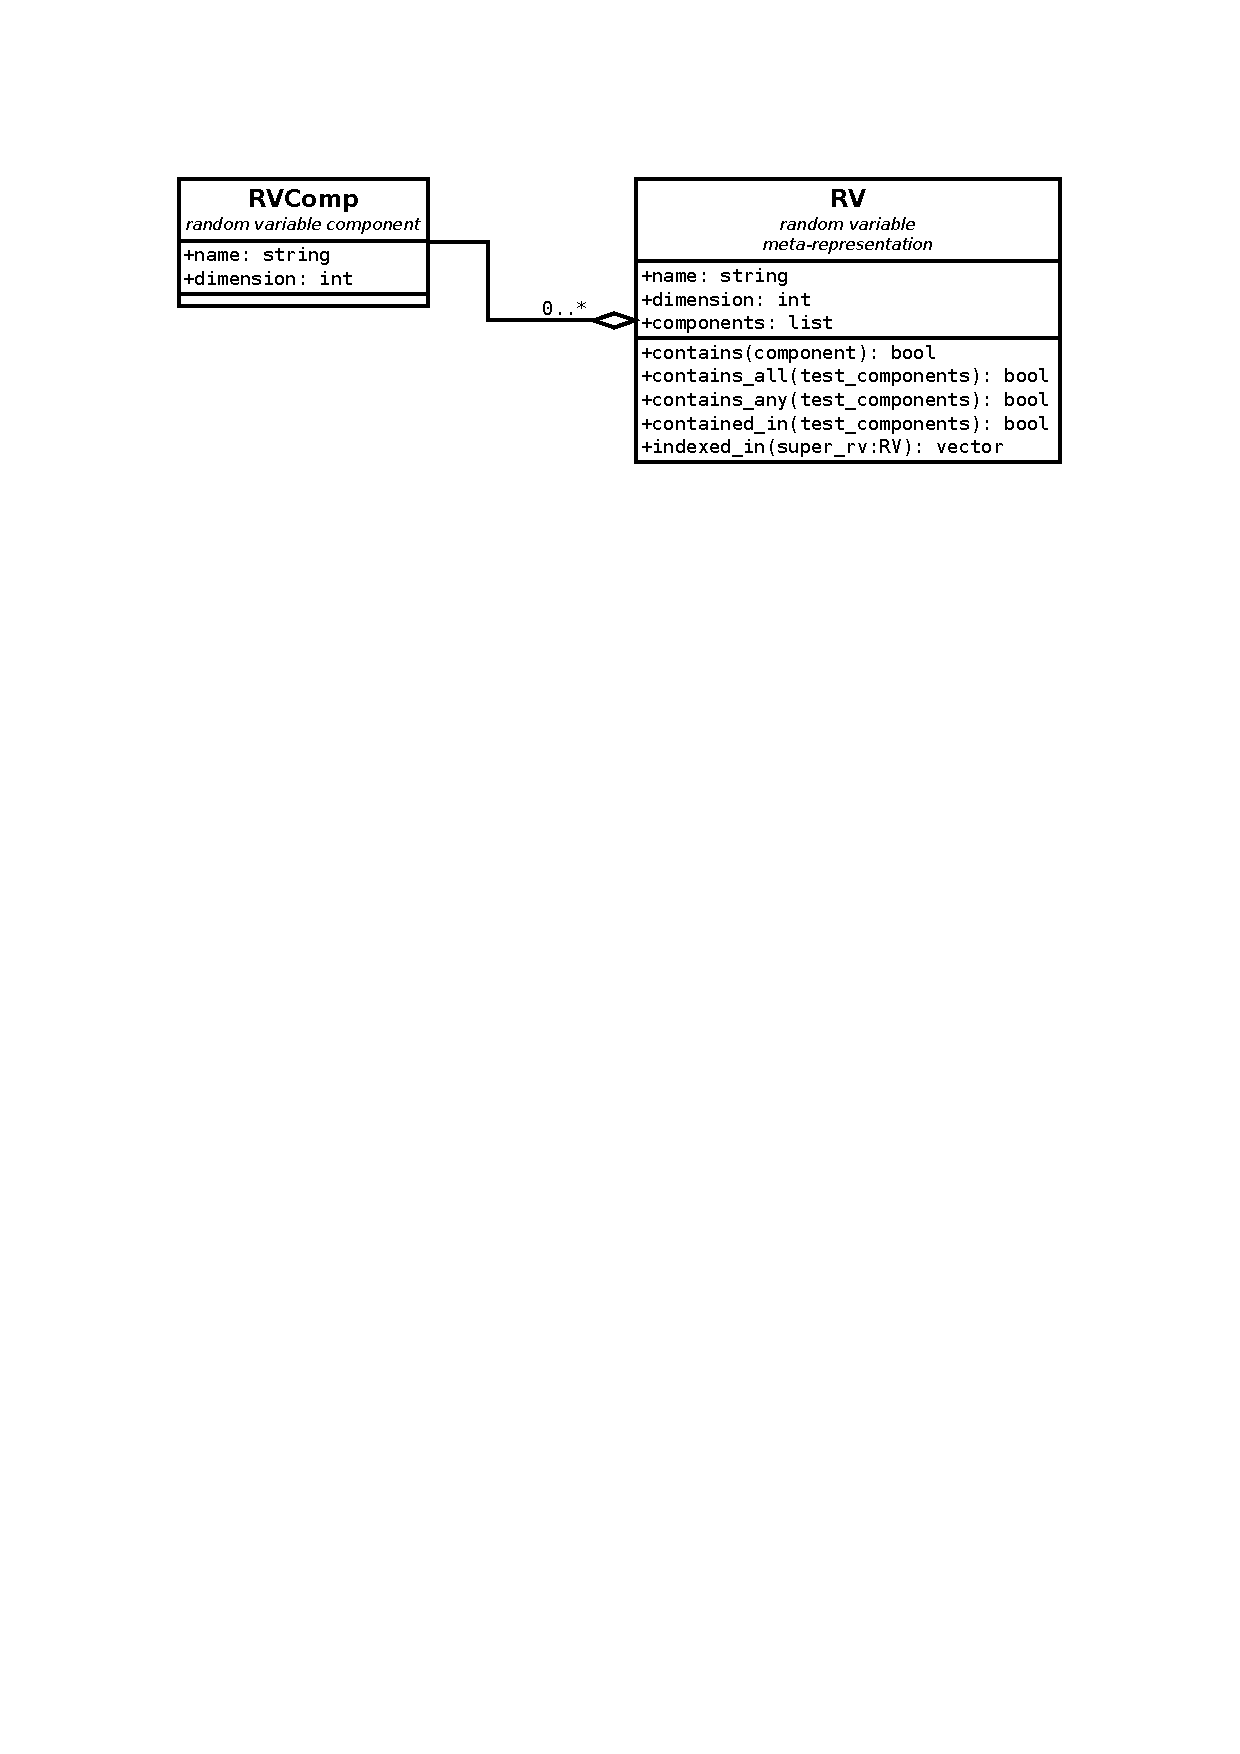
\includegraphics[width=\textwidth,keepaspectratio=true,clip=true,trim=3cm 218mm 3cm 3cm]{./diagrams/rvs.pdf}
	\vspace{-8mm}
	\caption{Class diagram of the random variable framework}
	\label{fig:DiaRvs}
\end{figure}

\subsection{Gaussian Probability Density Functions}

We continue by a brief mention of implemented {\pdfs}; our policy is to add new distributions on
as-needed basis rather than trying to have exhaustive set from the beginning. Every user of
PyBayes can create its own distributions by subclassing Pdf of CPdf and implementing meaningful
methods (there is no requirement for implementing unused methods).

PyBayes ships standard multivariate normal (Gaussian) {\pdf} through the \emph{GaussPdf} class;
related log-normal {\pdf} \emph{LogNormPdf} is also provided and shares common abstract superclass,
\emph{AbstractGaussPdf} with GaussPdf. The AbstractGaussPdf class only holds mean attribute \verb|mu|
and covariance matrix attribute \verb|R| and is useful mainly for the family of conditional Gaussian
{\pdfs} described below.

The most general conditional Gaussian distribution is the \emph{GaussCPdf} class that takes two
functions \verb|f| and \verb|g| as parameters plus the optional \verb|base_class| parameter in
constructor. The \verb|base_class| parameter defaults to GaussPdf, but can be set tu LogNormPdf (to
any AbstractGaussPdf subclass in general); the base class parameter determines resulting density ---
both conditional normal and log-normal distributions can be obtained without any code duplication,
thanks to abstraction provided by AbstractGaussPdf. GaussPdf transforms supplied condition \(c\)
using \eqref{eq:GaussCPdf}, substitutes to AbstractGaussPdf and calls respective \verb|base_class|
method.
\begin{equation} \label{eq:GaussCPdf}
	\begin{aligned}
		\mu &= f(c) \\
		R &= g(c)
	\end{aligned}
\end{equation}

First specialisation of GaussCPdf is the \emph{LinGaussCPdf} class that assumes that \verb|f| and
\verb|g| functions are linear, the transformation is thus according to \eqref{eq:LinGaussCPdf} where
condition is divided into parts \((c_1, c_2)\). The \verb|A|, \verb|C| (matrices), \verb|b| and
\verb|d| (vector) parameters are passed to the constructor. LinGaussCPdf exists mainly for
performance reasons and slightly higher convenience when passing arrays compared to functions;
LinGaussCPdf also benefits from generalisation offered AbstractGaussPdf.
\begin{equation} \label{eq:LinGaussCPdf}
	\begin{aligned}
		\mu &= A c_1 + b \\
		R &= C c_2 + d
	\end{aligned}
\end{equation}

The last GaussCPdf specialisation is the MLinGaussCPdf class which works almost identically as
LinGaussCPdf with the exception that the \verb|R| (covariance) parameter is fixed. Transformation
used by MLinGaussCPdf is thus defined by \eqref{eq:MLinGaussCPdf} where \(c\) is the conditioning
variable. MLinGaussCPdf also supports setting \verb|base_class| as usual.
\begin{equation} \label{eq:MLinGaussCPdf}
	\mu = A c + b
\end{equation}

See the \autoref{fig:DiaGaussPdfs} for a survey of Gaussian and related {\pdfs}.

\begin{figure}[h]
	\centering
	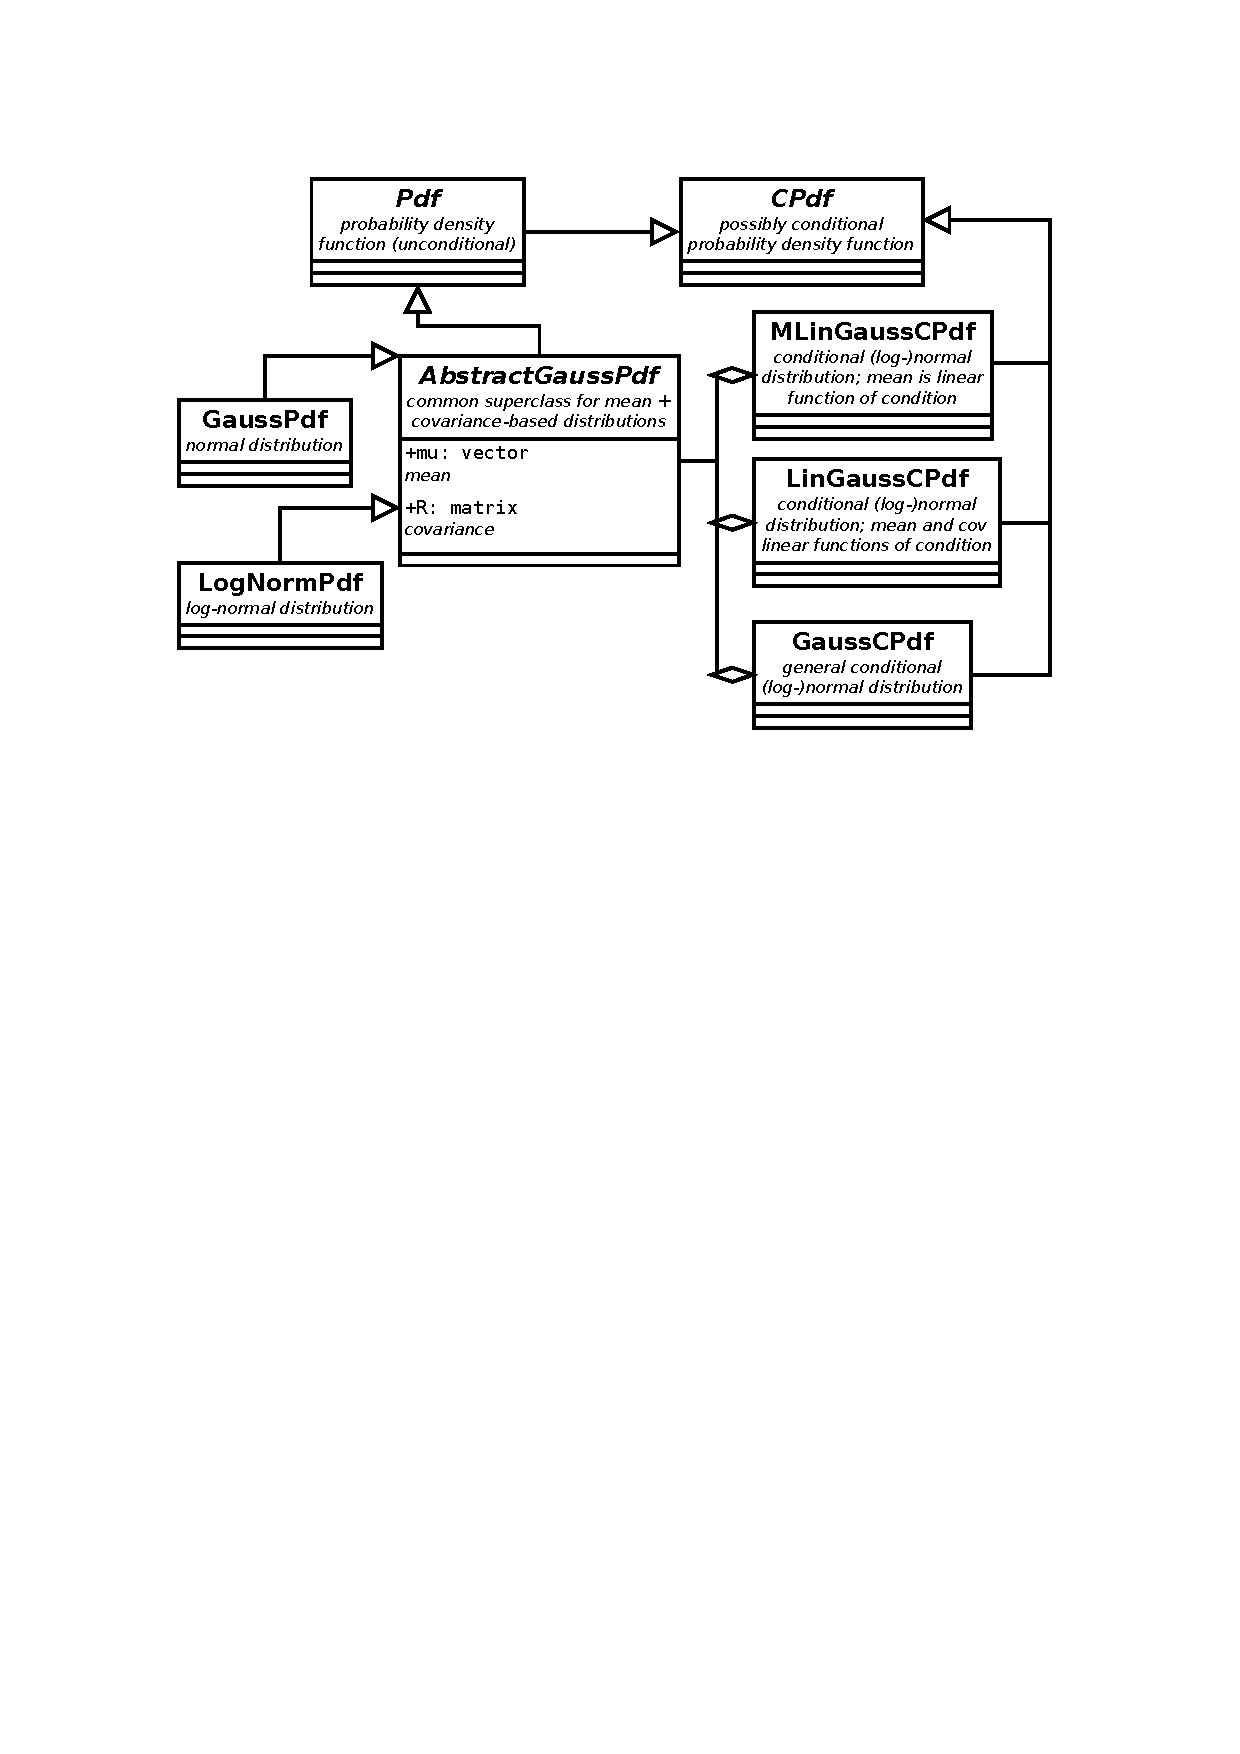
\includegraphics[width=\textwidth,keepaspectratio=true,clip=true,trim=3cm 173mm 3cm 3cm]{./diagrams/gaussian_pdfs.pdf}
	\vspace{-8mm}
	\caption{Class diagram of Gaussian and related distributions}
	\label{fig:DiaGaussPdfs}
\end{figure}

\subsection{Empirical Probability Density Functions}

Another very useful set of distributions is the empirical family suitable for particle filters.
Weighted empirical distribution named EmpPdf in PyBayes is the posterior {\pdf} of the
particle filter while a special product of weighted empirical distribution and a mixture of Gaussian
distributions is the posterior {\pdf} of the marginalized particle filter and is thus named
MarginalizedEmpPdf. Both inherit from AbstractEmpPdf in order to reuse code. Neither of the empirical
densities implement \verb|eval_log()| or \verb|sample()| --- while the latter would be possible, we
are yet to find a valid use-case for it (resampling particles being implemented differently).

The \emph{AbstractEmpPdf} class holds the \verb|weights| parameter, a vector of particle weights denoted as
\(\omega = (\omega_1, \omega_2 \dots \omega_n)\) in formulas. The usual constraints
\eqref{eq:AbstractEmpPdfConstraints} must hold. A simple method \verb|normalise_weights()| normalises
weights according to \eqref{eq:AbstractEmpPdfNormalise}.
\begin{align}
	\omega_i >= 0 \quad \forall i \quad \quad & \quad \quad \sum_{i=1}^n \omega_i = 1 \label{eq:AbstractEmpPdfConstraints} \\
	\omega_i' &= \frac{\omega_i}{\sum_{i=1}^n \omega_i} \label{eq:AbstractEmpPdfNormalise}
\end{align}
AbstractEmpPdf provides one more method, \verb|get_resample_indices()| which
(given that there are \(n\) particles) draws \(n\) random samples from itself and returns their
indices. The algorithm is however optimised in a way that only one random sampling is performed; the
results are thus more predictable (or, ``less random''), but this is desired when used for resampling
in particle filters --- its primary (and currently only) use.

The \emph{EmpPdf} class is the standard weighted empirical distribution \eqref{eq:EmpPdf} that extends
AbstractEmpPdf with the \verb|particles| attribute (a matrix) where each row \(x^{(i)}\) represents
one particle. It also provides the \verb|resample()| method that resamples particles using
\verb|get_resample_indices()| and resets weights to be uniformly distributed. EmpPdf has an extra
role in PyBayes, it is used to test \verb|sample()| of other {\pdfs} using the moment method
(sufficient number of samples is generated and sample mean and variance is compared with theoretical
results).
\begin{equation} \label{eq:EmpPdf}
	p(x) = \sum_{i=1}^n \omega_i \delta(x - x^{(i)})
\end{equation}

Related to the empirical density is the \emph{MarginalizedEmpPdf} that exists solely to form the
posterior {\pdf} of the marginalized particle filter. It extends AbstractEmpPdf with a vector of
GaussPdf objects \verb|gausses|, i-th GaussPdf is denoted as \(\mathcal{N}\left(\hat{a}^{(i)},
P^{(i)}\right)\) and a matrix \verb|particles| where i-th row is denoted as \(b^{(i)}\) in
\eqref{eq:MarginalizedEmpPdf}.
\begin{equation} \label{eq:MarginalizedEmpPdf}
	p(a, b) = \sum_{i=1}^n \omega_i \Big[ \mathcal{N}\left(\hat{a}^{(i)}, P^{(i)}\right) \Big]_a
		\delta(b - b^{(i)})
\end{equation}

MarginalizedEmpPdf doesn't provide a method for resampling as this task have to be done in the
particle filter implementation anyway at it has to deal also with the Kalman filters.

The class diagram of empirical {\pdfs} and related is displayed in the \autoref{fig:DiaEmpPdfs}.

\begin{figure}[h]
	\centering
	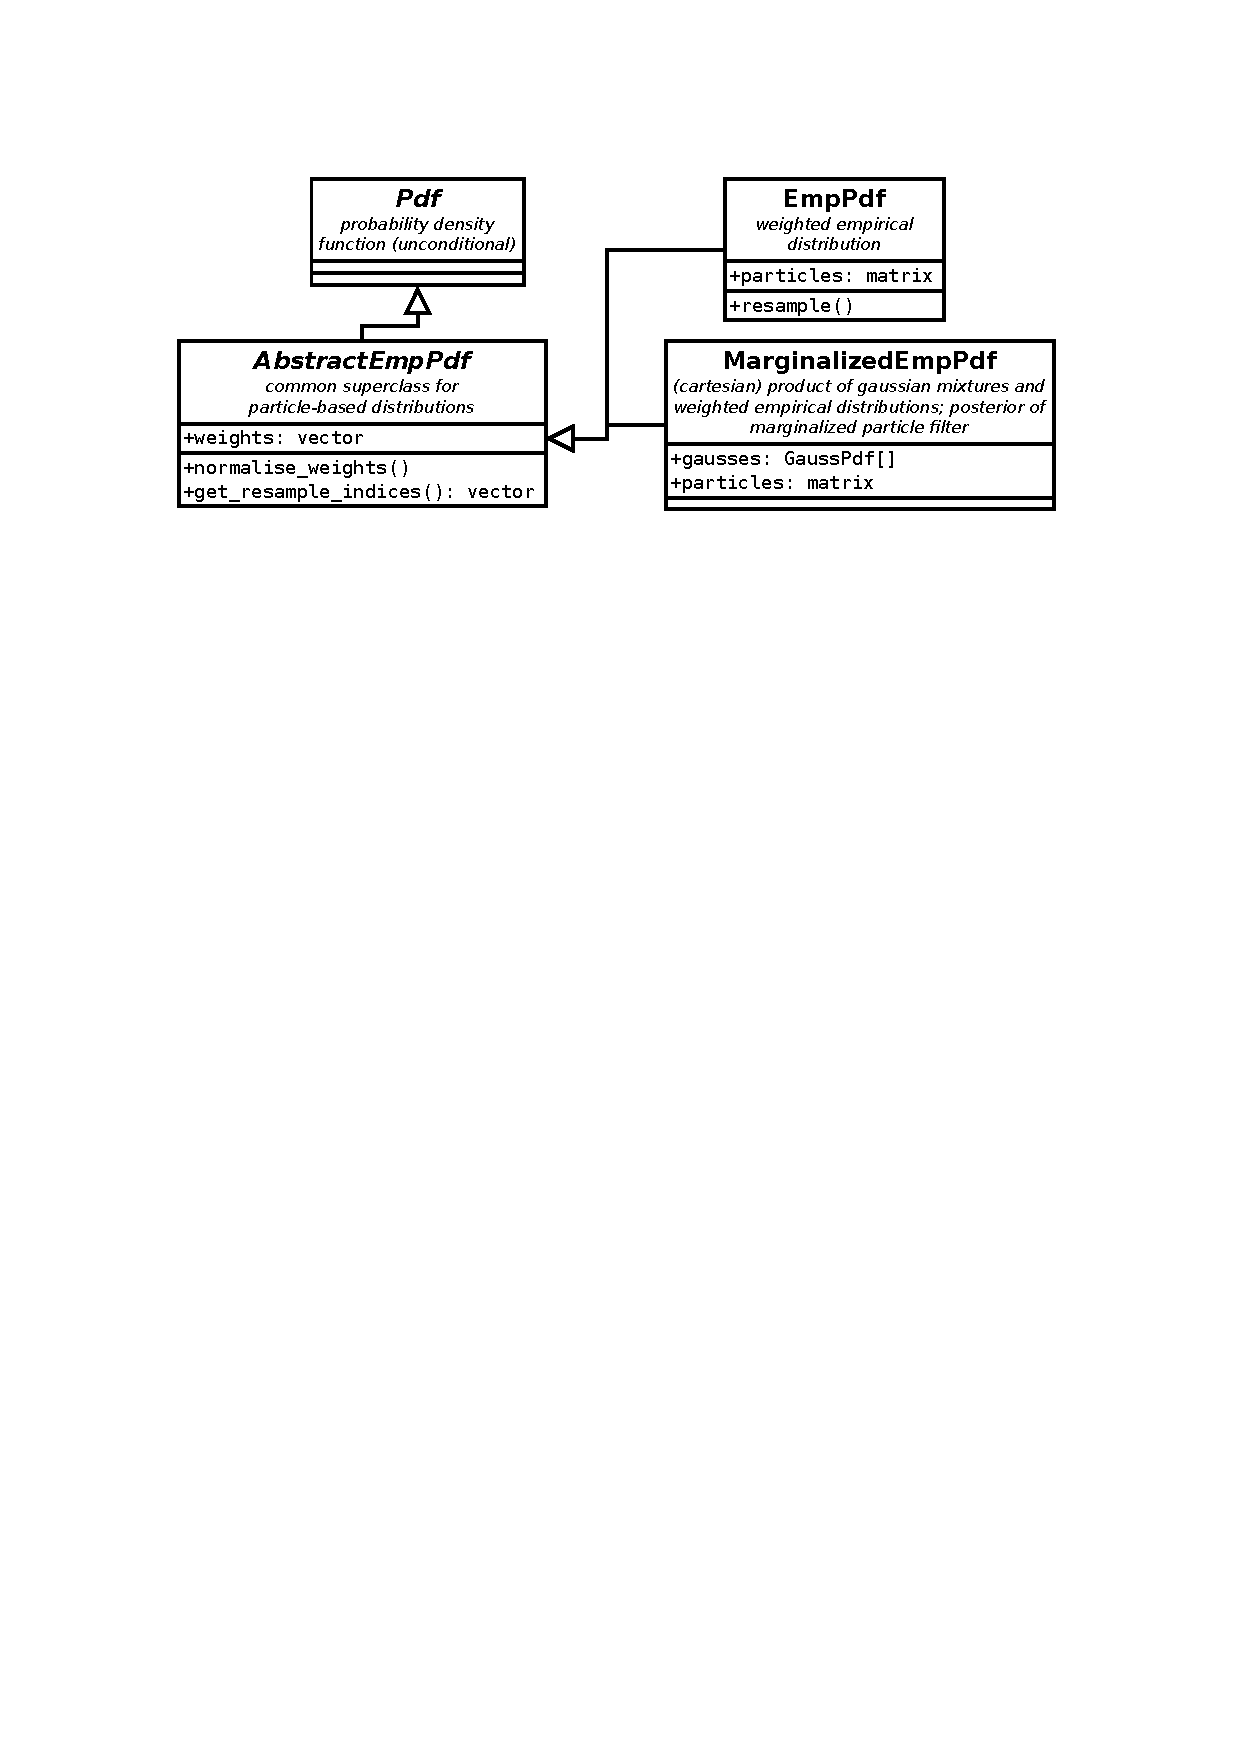
\includegraphics[width=\textwidth,keepaspectratio=true,clip=true,trim=3cm 210mm 3cm 3cm]{./diagrams/emp_pdfs.pdf}
	\vspace{-8mm}
	\caption{Class diagram of empirical distributions}
	\label{fig:DiaEmpPdfs}
\end{figure}

\subsection{Other Probability Density Functions}

We conclude the discussion about the implemented {\pdfs} with the ones that don't fit elsewhere.
|uniform pdf not mentioned elsewhere|

\subsection{Bayesian Filters}

[proposed citation: \cite{Smi:05}]

UML

Nice graph of a run of a particle filter (Mirda has the plotting code)

similar of marginalized particle filter? (gausses would be plotted vertically)

[mention this:\cite{Smi:10}]

\subsection{Wrappers} \label{sec:PyBayesWrappers}

about numpy, linalg wrappers, Tokyo...

\section{Documentation, Testing and Profiling} \label{sec:PyBayesDocsTests}

Documenting PyBayes using Sphinx, approach to documentation (mathematician-oriented), math in documentation

Testing - the separation of

- tests: test one class in isolation, quick, determinism (would be good, not achievable)

- stresses: test a great portion of code at once, run longer, non-determinism..

Note about coverage.py!!

Profiling python/cython - how, existing support in PyBayes

- how to correct profiling-induced overhead

\section{Performance Comparison with BDM} \label{sec:PyBayesPerformance}

[skip if in time press]
Python/Cython KalmanFilter, MATLAB oo / imperative / BDM

|see \autoref{fig:KF} (p. \pageref{fig:KF})|

\section{Discussion, Future Plans}

pypy + pure python mode
